\documentclass{article}\usepackage[]{graphicx}\usepackage[]{color}
%% maxwidth is the original width if it is less than linewidth
%% otherwise use linewidth (to make sure the graphics do not exceed the margin)
\makeatletter
\def\maxwidth{ %
  \ifdim\Gin@nat@width>\linewidth
    \linewidth
  \else
    \Gin@nat@width
  \fi
}
\makeatother

\definecolor{fgcolor}{rgb}{0.345, 0.345, 0.345}
\newcommand{\hlnum}[1]{\textcolor[rgb]{0.686,0.059,0.569}{#1}}%
\newcommand{\hlstr}[1]{\textcolor[rgb]{0.192,0.494,0.8}{#1}}%
\newcommand{\hlcom}[1]{\textcolor[rgb]{0.678,0.584,0.686}{\textit{#1}}}%
\newcommand{\hlopt}[1]{\textcolor[rgb]{0,0,0}{#1}}%
\newcommand{\hlstd}[1]{\textcolor[rgb]{0.345,0.345,0.345}{#1}}%
\newcommand{\hlkwa}[1]{\textcolor[rgb]{0.161,0.373,0.58}{\textbf{#1}}}%
\newcommand{\hlkwb}[1]{\textcolor[rgb]{0.69,0.353,0.396}{#1}}%
\newcommand{\hlkwc}[1]{\textcolor[rgb]{0.333,0.667,0.333}{#1}}%
\newcommand{\hlkwd}[1]{\textcolor[rgb]{0.737,0.353,0.396}{\textbf{#1}}}%
\let\hlipl\hlkwb

\usepackage{framed}
\makeatletter
\newenvironment{kframe}{%
 \def\at@end@of@kframe{}%
 \ifinner\ifhmode%
  \def\at@end@of@kframe{\end{minipage}}%
  \begin{minipage}{\columnwidth}%
 \fi\fi%
 \def\FrameCommand##1{\hskip\@totalleftmargin \hskip-\fboxsep
 \colorbox{shadecolor}{##1}\hskip-\fboxsep
     % There is no \\@totalrightmargin, so:
     \hskip-\linewidth \hskip-\@totalleftmargin \hskip\columnwidth}%
 \MakeFramed {\advance\hsize-\width
   \@totalleftmargin\z@ \linewidth\hsize
   \@setminipage}}%
 {\par\unskip\endMakeFramed%
 \at@end@of@kframe}
\makeatother

\definecolor{shadecolor}{rgb}{.97, .97, .97}
\definecolor{messagecolor}{rgb}{0, 0, 0}
\definecolor{warningcolor}{rgb}{1, 0, 1}
\definecolor{errorcolor}{rgb}{1, 0, 0}
\newenvironment{knitrout}{}{} % an empty environment to be redefined in TeX

\usepackage{alltt}

\usepackage{amsmath, amssymb}
\usepackage{graphicx}
\usepackage{hyperref}
\IfFileExists{upquote.sty}{\usepackage{upquote}}{}
\begin{document}

\title{Pol Sci 630:  Problem Set 12 Solutions: Heteroskedasticity, Autocorrelation}

\author{Prepared by: Anh Le (\href{mailto:anh.le@duke.edu}{anh.le@duke.edu})}

\date{Due Date: Friday, Nov 20, 2015, 12 AM (Beginning of Lab)}

\maketitle

\begin{knitrout}
\definecolor{shadecolor}{rgb}{0.969, 0.969, 0.969}\color{fgcolor}\begin{kframe}
\begin{alltt}
\hlkwd{rm}\hlstd{(}\hlkwc{list} \hlstd{=} \hlkwd{ls}\hlstd{())}
\hlkwd{library}\hlstd{(ggplot2)}
\end{alltt}
\end{kframe}
\end{knitrout}


\section{Heteroskedasticity}

This exercise nudges you to think about heteroskedasticity as a theoretical / social science problem, not a mechanical / statistical issue to be blindly fixed.

One common cause of heteroskedasticity is that our model does not take into account heterogenous effect across sub-populations. For example, we have a model of spending (dependent var) as a function of income (independent var), and the propensity to spend differs across ethnic groups. Formally,

\begin{align}
spending &= \beta_{ethnic} income + \epsilon
\end{align}

where $\beta_{ethnic}$ takes a different value for white, black, and asian. If we don't know about this heterogeneity of propensity to spend across ethnic groups, the graph will show heteroskedasticity:

\begin{knitrout}
\definecolor{shadecolor}{rgb}{0.969, 0.969, 0.969}\color{fgcolor}
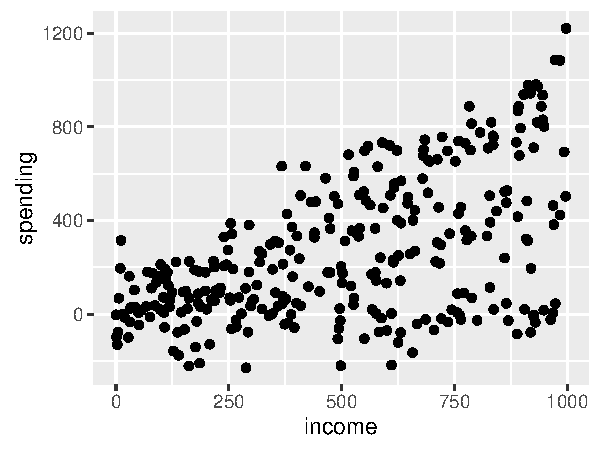
\includegraphics[width=\maxwidth]{figure/unnamed-chunk-2-1} 

\end{knitrout}

Buf if we are smart researcher, we'll realize the underlying cause of the heterogeneity, as shown in the following plot:

\begin{knitrout}
\definecolor{shadecolor}{rgb}{0.969, 0.969, 0.969}\color{fgcolor}
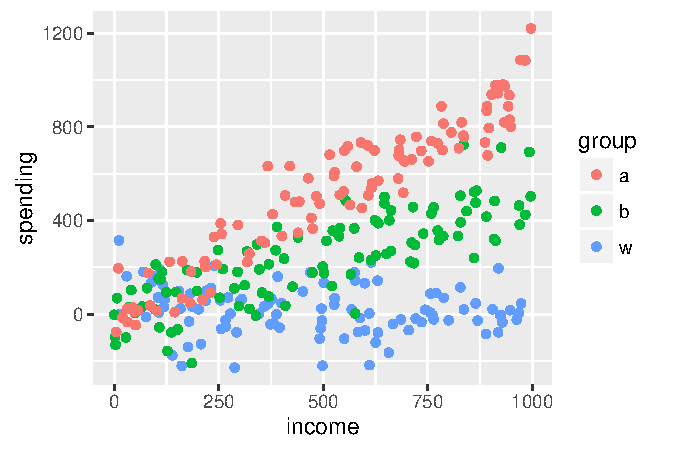
\includegraphics[width=\maxwidth]{figure/unnamed-chunk-3-1} 

\end{knitrout}

The take-home point is that heteroskedasticity could be a signal of underlying model specification, and we should think hard about the cause of heteroskedasticity instead of applying a quick fix.

\subsection{Simulating}

Simulate the spending and income pattern for three ethnic groups as described above. Re-create the two plots above. The numbers don't have to be the same -- just make sure that your data has heteroskedasticity due to underlying heterogenous effect across ethnic groups as described in the example above. Note: Don't look at my code.

\subsection{Diagnostics: Visual}

Using the simulated data above, regress spending on income, plot the residual against the predicted value.

\textbf{Solution}

\begin{knitrout}
\definecolor{shadecolor}{rgb}{0.969, 0.969, 0.969}\color{fgcolor}\begin{kframe}
\begin{alltt}
\hlstd{m_het} \hlkwb{<-} \hlkwd{lm}\hlstd{(spending} \hlopt{~} \hlstd{income,} \hlkwc{data} \hlstd{= d)}
\hlkwd{plot}\hlstd{(}\hlkwd{predict}\hlstd{(m_het),} \hlkwd{resid}\hlstd{(m_het))}
\end{alltt}
\end{kframe}
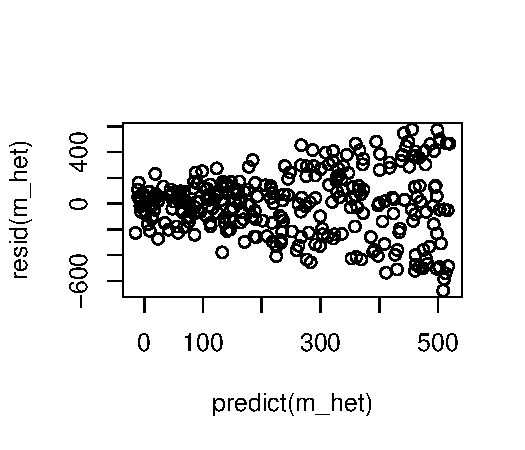
\includegraphics[width=\maxwidth]{figure/unnamed-chunk-4-1} 

\end{knitrout}

\subsection{Diagonistics: Hypothesis test}

Conduct BP test and White test. Why do the tests reach the same conclusion here, unlike in the lab tutorial?

\textbf{Solution}

\begin{knitrout}
\definecolor{shadecolor}{rgb}{0.969, 0.969, 0.969}\color{fgcolor}\begin{kframe}
\begin{alltt}
\hlkwd{library}\hlstd{(AER)}
\hlkwd{bptest}\hlstd{(m_het,} \hlkwc{varformula} \hlstd{=} \hlopt{~} \hlstd{income,} \hlkwc{data} \hlstd{= d)}
\end{alltt}
\begin{verbatim}
## 
## 	studentized Breusch-Pagan test
## 
## data:  m_het
## BP = 95.706, df = 1, p-value < 2.2e-16
\end{verbatim}
\begin{alltt}
\hlkwd{bptest}\hlstd{(m_het,} \hlkwc{varformula} \hlstd{=} \hlopt{~} \hlstd{income} \hlopt{+} \hlkwd{I}\hlstd{(income}\hlopt{^}\hlnum{2}\hlstd{),} \hlkwc{data} \hlstd{= d)}
\end{alltt}
\begin{verbatim}
## 
## 	studentized Breusch-Pagan test
## 
## data:  m_het
## BP = 103.16, df = 2, p-value < 2.2e-16
\end{verbatim}
\end{kframe}
\end{knitrout}

The test reaches the same conclusion because the variance of the error terms is a linear function of $income$ (not of $income^2$, for example), so both the BP and the White tests are able to detect this.

\subsection{Diagnostics: Repeat the White's test manually}

Here's the instruction. Compare the result you get doing it by hand vs using R.

\textit{White test (Wooldridge "Introductory", Testing for heteroskedasticity)}

1. Estimate the model \verb`y ~ x_1 + x_2 + ... + x_k` by OLS, as usual. Obtain the OLS residual $\hat u$ and the fitted values $\hat y$. Compute $\hat u^2$ and $\hat y^2$.

2. Run the regression $\hat u^2 = \delta_0 + \delta_1 \hat y + \delta_2 \hat y^2$. Keep the R square.

3. \textbf{I want you to use the LM for this problem} Form either the F or LM statistic and compute the p-value (using the $F_{2,n-3}$ distribution in the former case and the $\chi_2^2$ distribution in the latter case).

\textbf{Solution}

\begin{knitrout}
\definecolor{shadecolor}{rgb}{0.969, 0.969, 0.969}\color{fgcolor}\begin{kframe}
\begin{alltt}
\hlstd{uhat} \hlkwb{<-} \hlkwd{resid}\hlstd{(m_het) ; yhat} \hlkwb{<-} \hlkwd{predict}\hlstd{(m_het)}
\hlstd{m_white_stage2} \hlkwb{<-} \hlkwd{lm}\hlstd{(}\hlkwd{I}\hlstd{(uhat}\hlopt{^}\hlnum{2}\hlstd{)} \hlopt{~} \hlstd{yhat} \hlopt{+} \hlkwd{I}\hlstd{(yhat}\hlopt{^}\hlnum{2}\hlstd{))}
\hlstd{R_squared} \hlkwb{<-} \hlkwd{summary}\hlstd{(m_white_stage2)}\hlopt{$}\hlstd{r.squared}

\hlstd{n} \hlkwb{<-} \hlkwd{nrow}\hlstd{(d) ; k} \hlkwb{<-} \hlnum{2} \hlcom{# k = 1 because we have 2 regressors, yhat and yhat squared}
\hlstd{(LM_stat} \hlkwb{<-} \hlstd{n} \hlopt{*} \hlstd{R_squared)}
\end{alltt}
\begin{verbatim}
## [1] 103.157
\end{verbatim}
\begin{alltt}
\hlnum{1} \hlopt{-} \hlstd{(pvalue} \hlkwb{<-} \hlkwd{pchisq}\hlstd{(LM_stat,} \hlkwc{df} \hlstd{= k))}
\end{alltt}
\begin{verbatim}
## [1] 0
\end{verbatim}
\begin{alltt}
\hlkwd{bptest}\hlstd{(m_het,} \hlkwc{varformula} \hlstd{=} \hlopt{~} \hlstd{yhat} \hlopt{+} \hlkwd{I}\hlstd{(yhat}\hlopt{^}\hlnum{2}\hlstd{),} \hlkwc{data} \hlstd{= d)}
\end{alltt}
\begin{verbatim}
## 
## 	studentized Breusch-Pagan test
## 
## data:  m_het
## BP = 103.16, df = 2, p-value < 2.2e-16
\end{verbatim}
\end{kframe}
\end{knitrout}

The LM statistic and the p value are the same.

\subsection{Fixing: robust standard error}

Run hypothesis test without and with robust standard error. What's the conclusion?

\textbf{Solution}

\begin{knitrout}
\definecolor{shadecolor}{rgb}{0.969, 0.969, 0.969}\color{fgcolor}\begin{kframe}
\begin{alltt}
\hlkwd{summary}\hlstd{(m_het)}
\end{alltt}
\begin{verbatim}
## 
## Call:
## lm(formula = spending ~ income, data = d)
## 
## Residuals:
##     Min      1Q  Median      3Q     Max 
## -675.87 -149.60   19.05  135.80  576.52 
## 
## Coefficients:
##              Estimate Std. Error t value Pr(>|t|)    
## (Intercept) -17.82943   26.56899  -0.671    0.503    
## income        0.53868    0.04639  11.611   <2e-16 ***
## ---
## Signif. codes:  0 '***' 0.001 '**' 0.01 '*' 0.05 '.' 0.1 ' ' 1
## 
## Residual standard error: 243.8 on 298 degrees of freedom
## Multiple R-squared:  0.3115,	Adjusted R-squared:  0.3092 
## F-statistic: 134.8 on 1 and 298 DF,  p-value: < 2.2e-16
\end{verbatim}
\begin{alltt}
\hlkwd{coeftest}\hlstd{(m_het,} \hlkwc{vcov} \hlstd{=} \hlkwd{vcovHC}\hlstd{(m_het,} \hlkwc{type} \hlstd{=} \hlstr{"HC"}\hlstd{))}
\end{alltt}
\begin{verbatim}
## 
## t test of coefficients:
## 
##               Estimate Std. Error t value Pr(>|t|)    
## (Intercept) -17.829433  18.463054 -0.9657    0.335    
## income        0.538684   0.051638 10.4319   <2e-16 ***
## ---
## Signif. codes:  0 '***' 0.001 '**' 0.01 '*' 0.05 '.' 0.1 ' ' 1
\end{verbatim}
\end{kframe}
\end{knitrout}

Both regressions show that income has a positive and significant impact on spending

\subsection{Fixing: robust standard error by hand}

\textbf{Solution}

\begin{knitrout}
\definecolor{shadecolor}{rgb}{0.969, 0.969, 0.969}\color{fgcolor}\begin{kframe}
\begin{alltt}
\hlstd{m_robust1} \hlkwb{<-} \hlkwd{lm}\hlstd{(income} \hlopt{~} \hlnum{1}\hlstd{,} \hlkwc{data} \hlstd{= d)}
\hlstd{numerator} \hlkwb{<-} \hlkwd{sum}\hlstd{((}\hlkwd{resid}\hlstd{(m_robust1)}\hlopt{**}\hlnum{2}\hlstd{)} \hlopt{*} \hlstd{(}\hlkwd{resid}\hlstd{(m_het)}\hlopt{**}\hlnum{2}\hlstd{))}
\hlstd{SSR} \hlkwb{<-} \hlkwd{sum}\hlstd{(}\hlkwd{resid}\hlstd{(m_robust1)}\hlopt{**}\hlnum{2}\hlstd{)} \hlopt{**} \hlnum{2}

\hlcom{# Compare the two methods}
\hlstd{(var_beta_x} \hlkwb{<-} \hlstd{numerator} \hlopt{/} \hlstd{SSR)}
\end{alltt}
\begin{verbatim}
## [1] 0.002666474
\end{verbatim}
\begin{alltt}
\hlkwd{vcovHC}\hlstd{(m_het,} \hlkwc{type} \hlstd{=} \hlstr{"HC"}\hlstd{)}
\end{alltt}
\begin{verbatim}
##             (Intercept)       income
## (Intercept)   340.88438 -0.795780000
## income         -0.79578  0.002666474
\end{verbatim}
\end{kframe}
\end{knitrout}

We see that the manual method and R's \verb`vcovHC` gives the same robust standard error.

\subsection{Fixing: Provide a correct model}

Specify a regression model that takes into account heterogenous effect of income on spending across ethnic groups. Show that there's no longer heteroskedasticity.

\textbf{Solution}

\begin{knitrout}
\definecolor{shadecolor}{rgb}{0.969, 0.969, 0.969}\color{fgcolor}\begin{kframe}
\begin{alltt}
\hlstd{m_group} \hlkwb{<-} \hlkwd{lm}\hlstd{(spending} \hlopt{~} \hlstd{income} \hlopt{+} \hlstd{group} \hlopt{+} \hlstd{income}\hlopt{:}\hlstd{group,} \hlkwc{data} \hlstd{= d)}
\hlkwd{plot}\hlstd{(}\hlkwd{resid}\hlstd{(m_group)} \hlopt{~} \hlkwd{predict}\hlstd{(m_group))}
\end{alltt}
\end{kframe}
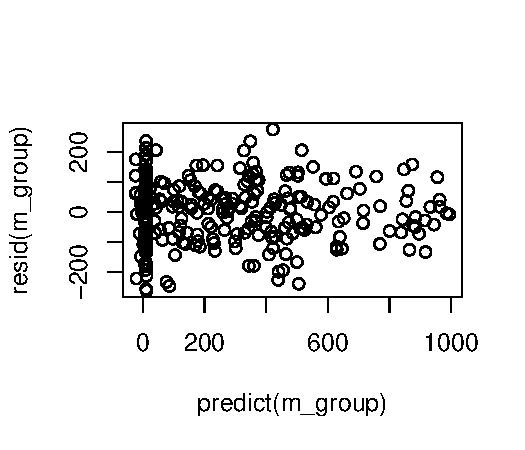
\includegraphics[width=\maxwidth]{figure/unnamed-chunk-9-1} 

\end{knitrout}

As shown in the diagnostics plot, there's no longer heteroskedasticity

\end{document}
